
%% bare_conf.tex
%% V1.3
%% 2007/01/11
%% by Michael Shell
%% See:
%% http://www.michaelshell.org/
%% for current contact information.
%%
%% This is a skeleton file demonstrating the use of IEEEtran.cls
%% (requires IEEEtran.cls version 1.7 or later) with an IEEE conference paper.
%%
%% Support sites:
%% http://www.michaelshell.org/tex/ieeetran/
%% http://www.ctan.org/tex-archive/macros/latex/contrib/IEEEtran/
%% and
%% http://www.ieee.org/

%%*************************************************************************
%% Legal Notice:
%% This code is offered as-is without any warranty either expressed or
%% implied; without even the implied warranty of MERCHANTABILITY or
%% FITNESS FOR A PARTICULAR PURPOSE! 
%% User assumes all risk.
%% In no event shall IEEE or any contributor to this code be liable for
%% any damages or losses, including, but not limited to, incidental,
%% consequential, or any other damages, resulting from the use or misuse
%% of any information contained here.
%%
%% All comments are the opinions of their respective authors and are not
%% necessarily endorsed by the IEEE.
%%
%% This work is distributed under the LaTeX Project Public License (LPPL)
%% ( http://www.latex-project.org/ ) version 1.3, and may be freely used,
%% distributed and modified. A copy of the LPPL, version 1.3, is included
%% in the base LaTeX documentation of all distributions of LaTeX released
%% 2003/12/01 or later.
%% Retain all contribution notices and credits.
%% ** Modified files should be clearly indicated as such, including  **
%% ** renaming them and changing author support contact information. **
%%
%% File list of work: IEEEtran.cls, IEEEtran_HOWTO.pdf, bare_adv.tex,
%%                    bare_conf.tex, bare_jrnl.tex, bare_jrnl_compsoc.tex
%%*************************************************************************

% *** Authors should verify (and, if needed, correct) their LaTeX system  ***
% *** with the testflow diagnostic prior to trusting their LaTeX platform ***
% *** with production work. IEEE's font choices can trigger bugs that do  ***
% *** not appear when using other class files.                            ***
% The testflow support page is at:
% http://www.michaelshell.org/tex/testflow/



% Note that the a4paper option is mainly intended so that authors in
% countries using A4 can easily print to A4 and see how their papers will
% look in print - the typesetting of the document will not typically be
% affected with changes in paper size (but the bottom and side margins will).
% Use the testflow package mentioned above to verify correct handling of
% both paper sizes by the user's LaTeX system.
%
% Also note that the "draftcls" or "draftclsnofoot", not "draft", option
% should be used if it is desired that the figures are to be displayed in
% draft mode.
%
\documentclass[10pt, conference, compsocconf]{IEEEtran}
\usepackage[utf8]{inputenc}
\usepackage[brazil]{babel}
% Add the compsocconf option for Computer Society conferences.
%
% If IEEEtran.cls has not been installed into the LaTeX system files,
% manually specify the path to it like:
% \documentclass[conference]{../sty/IEEEtran}


% Some very useful LaTeX packages include:
% (uncomment the ones you want to load)


% *** MISC UTILITY PACKAGES ***
%
%\usepackage{ifpdf}
% Heiko Oberdiek's ifpdf.sty is very useful if you need conditional
% compilation based on whether the output is pdf or dvi.
% usage:
% \ifpdf
%   % pdf code
% \else
%   % dvi code
% \fi
% The latest version of ifpdf.sty can be obtained from:
% http://www.ctan.org/tex-archive/macros/latex/contrib/oberdiek/
% Also, note that IEEEtran.cls V1.7 and later provides a builtin
% \ifCLASSINFOpdf conditional that works the same way.
% When switching from latex to pdflatex and vice-versa, the compiler may
% have to be run twice to clear warning/error messages.


% *** CITATION PACKAGES ***
%
\usepackage{cite}
% cite.sty was written by Donald Arseneau
% V1.6 and later of IEEEtran pre-defines the format of the cite.sty package
% \cite{} output to follow that of IEEE. Loading the cite package will
% result in citation numbers being automatically sorted and properly
% "compressed/ranged". e.g., [1], [9], [2], [7], [5], [6] without using
% cite.sty will become [1], [2], [5]--[7], [9] using cite.sty. cite.sty's
% \cite will automatically add leading space, if needed. Use cite.sty's
% noadjust option (cite.sty V3.8 and later) if you want to turn this off.
% cite.sty is already installed on most LaTeX systems. Be sure and use
% version 4.0 (2003-05-27) and later if using hyperref.sty. cite.sty does
% not currently provide for hyperlinked citations.
% The latest version can be obtained at:
% http://www.ctan.org/tex-archive/macros/latex/contrib/cite/
% The documentation is contained in the cite.sty file itself.






% *** GRAPHICS RELATED PACKAGES ***
%
\ifCLASSINFOpdf
   \usepackage[pdftex]{graphicx}
  % declare the path(s) where your graphic files are
  % \graphicspath{{../pdf/}{../jpeg/}}
  % and their extensions so you won't have to specify these with
  % every instance of \includegraphics
  \DeclareGraphicsExtensions{.pdf,.jpeg,.png}
\else
  % or other class option (dvipsone, dvipdf, if not using dvips). graphicx
  % will default to the driver specified in the system graphics.cfg if no
  % driver is specified.
  % \usepackage[dvips]{graphicx}
  % declare the path(s) where your graphic files are
  % \graphicspath{{../eps/}}
  % and their extensions so you won't have to specify these with
  % every instance of \includegraphics
  % \DeclareGraphicsExtensions{.eps}
\fi
% graphicx was written by David Carlisle and Sebastian Rahtz. It is
% required if you want graphics, photos, etc. graphicx.sty is already
% installed on most LaTeX systems. The latest version and documentation can
% be obtained at: 
% http://www.ctan.org/tex-archive/macros/latex/required/graphics/
% Another good source of documentation is "Using Imported Graphics in
% LaTeX2e" by Keith Reckdahl which can be found as epslatex.ps or
% epslatex.pdf at: http://www.ctan.org/tex-archive/info/
%
% latex, and pdflatex in dvi mode, support graphics in encapsulated
% postscript (.eps) format. pdflatex in pdf mode supports graphics
% in .pdf, .jpeg, .png and .mps (metapost) formats. Users should ensure
% that all non-photo figures use a vector format (.eps, .pdf, .mps) and
% not a bitmapped formats (.jpeg, .png). IEEE frowns on bitmapped formats
% which can result in "jaggedy"/blurry rendering of lines and letters as
% well as large increases in file sizes.
%
% You can find documentation about the pdfTeX application at:
% http://www.tug.org/applications/pdftex





% *** MATH PACKAGES ***
%
\usepackage[cmex10]{amsmath}
% A popular package from the American Mathematical Society that provides
% many useful and powerful commands for dealing with mathematics. If using
% it, be sure to load this package with the cmex10 option to ensure that
% only type 1 fonts will utilized at all point sizes. Without this option,
% it is possible that some math symbols, particularly those within
% footnotes, will be rendered in bitmap form which will result in a
% document that can not be IEEE Xplore compliant!
%
% Also, note that the amsmath package sets \interdisplaylinepenalty to 10000
% thus preventing page breaks from occurring within multiline equations. Use:
\interdisplaylinepenalty=2500
% after loading amsmath to restore such page breaks as IEEEtran.cls normally
% does. amsmath.sty is already installed on most LaTeX systems. The latest
% version and documentation can be obtained at:
% http://www.ctan.org/tex-archive/macros/latex/required/amslatex/math/





% *** SPECIALIZED LIST PACKAGES ***
%
\usepackage{algorithmic}
% algorithmic.sty was written by Peter Williams and Rogerio Brito.
% This package provides an algorithmic environment fo describing algorithms.
% You can use the algorithmic environment in-text or within a figure
% environment to provide for a floating algorithm. Do NOT use the algorithm
% floating environment provided by algorithm.sty (by the same authors) or
% algorithm2e.sty (by Christophe Fiorio) as IEEE does not use dedicated
% algorithm float types and packages that provide these will not provide
% correct IEEE style captions. The latest version and documentation of
% algorithmic.sty can be obtained at:
% http://www.ctan.org/tex-archive/macros/latex/contrib/algorithms/
% There is also a support site at:
% http://algorithms.berlios.de/index.html
% Also of interest may be the (relatively newer and more customizable)
% algorithmicx.sty package by Szasz Janos:
% http://www.ctan.org/tex-archive/macros/latex/contrib/algorithmicx/




% *** ALIGNMENT PACKAGES ***
%
%\usepackage{array}
% Frank Mittelbach's and David Carlisle's array.sty patches and improves
% the standard LaTeX2e array and tabular environments to provide better
% appearance and additional user controls. As the default LaTeX2e table
% generation code is lacking to the point of almost being broken with
% respect to the quality of the end results, all users are strongly
% advised to use an enhanced (at the very least that provided by array.sty)
% set of table tools. array.sty is already installed on most systems. The
% latest version and documentation can be obtained at:
% http://www.ctan.org/tex-archive/macros/latex/required/tools/


%\usepackage{mdwmath}
%\usepackage{mdwtab}
% Also highly recommended is Mark Wooding's extremely powerful MDW tools,
% especially mdwmath.sty and mdwtab.sty which are used to format equations
% and tables, respectively. The MDWtools set is already installed on most
% LaTeX systems. The lastest version and documentation is available at:
% http://www.ctan.org/tex-archive/macros/latex/contrib/mdwtools/


% IEEEtran contains the IEEEeqnarray family of commands that can be used to
% generate multiline equations as well as matrices, tables, etc., of high
% quality.


%\usepackage{eqparbox}
% Also of notable interest is Scott Pakin's eqparbox package for creating
% (automatically sized) equal width boxes - aka "natural width parboxes".
% Available at:
% http://www.ctan.org/tex-archive/macros/latex/contrib/eqparbox/





% *** SUBFIGURE PACKAGES ***
\usepackage[tight,footnotesize]{subfigure}

% subfigure.sty was written by Steven Douglas Cochran. This package makes it
% easy to put subfigures in your figures. e.g., "Figure 1a and 1b". For IEEE
% work, it is a good idea to load it with the tight package option to reduce
% the amount of white space around the subfigures. subfigure.sty is already
% installed on most LaTeX systems. The latest version and documentation can
% be obtained at:
% http://www.ctan.org/tex-archive/obsolete/macros/latex/contrib/subfigure/
% subfigure.sty has been superceeded by subfig.sty.

%\usepackage[caption=false]{caption}
\usepackage[font=footnotesize]{subfig}
% subfig.sty, also written by Steven Douglas Cochran, is the modern
% replacement for subfigure.sty. However, subfig.sty requires and
% automatically loads Axel Sommerfeldt's caption.sty which will override
% IEEEtran.cls handling of captions and this will result in nonIEEE style
% figure/table captions. To prevent this problem, be sure and preload
% caption.sty with its "caption=false" package option. This is will preserve
% IEEEtran.cls handing of captions. Version 1.3 (2005/06/28) and later 
% (recommended due to many improvements over 1.2) of subfig.sty supports
% the caption=false option directly:
%\usepackage[caption=false,font=footnotesize]{subfig}
%
% The latest version and documentation can be obtained at:
% http://www.ctan.org/tex-archive/macros/latex/contrib/subfig/
% The latest version and documentation of caption.sty can be obtained at:
% http://www.ctan.org/tex-archive/macros/latex/contrib/caption/




% *** FLOAT PACKAGES ***
%
%\usepackage{fixltx2e}
% fixltx2e, the successor to the earlier fix2col.sty, was written by
% Frank Mittelbach and David Carlisle. This package corrects a few problems
% in the LaTeX2e kernel, the most notable of which is that in current
% LaTeX2e releases, the ordering of single and double column floats is not
% guaranteed to be preserved. Thus, an unpatched LaTeX2e can allow a
% single column figure to be placed prior to an earlier double column
% figure. The latest version and documentation can be found at:
% http://www.ctan.org/tex-archive/macros/latex/base/



%\usepackage{stfloats}
% stfloats.sty was written by Sigitas Tolusis. This package gives LaTeX2e
% the ability to do double column floats at the bottom of the page as well
% as the top. (e.g., "\begin{figure*}[!b]" is not normally possible in
% LaTeX2e). It also provides a command:
%\fnbelowfloat
% to enable the placement of footnotes below bottom floats (the standard
% LaTeX2e kernel puts them above bottom floats). This is an invasive package
% which rewrites many portions of the LaTeX2e float routines. It may not work
% with other packages that modify the LaTeX2e float routines. The latest
% version and documentation can be obtained at:
% http://www.ctan.org/tex-archive/macros/latex/contrib/sttools/
% Documentation is contained in the stfloats.sty comments as well as in the
% presfull.pdf file. Do not use the stfloats baselinefloat ability as IEEE
% does not allow \baselineskip to stretch. Authors submitting work to the
% IEEE should note that IEEE rarely uses double column equations and
% that authors should try to avoid such use. Do not be tempted to use the
% cuted.sty or midfloat.sty packages (also by Sigitas Tolusis) as IEEE does
% not format its papers in such ways.





% *** PDF, URL AND HYPERLINK PACKAGES ***
%
%\usepackage{url}
% url.sty was written by Donald Arseneau. It provides better support for
% handling and breaking URLs. url.sty is already installed on most LaTeX
% systems. The latest version can be obtained at:
% http://www.ctan.org/tex-archive/macros/latex/contrib/misc/
% Read the url.sty source comments for usage information. Basically,
% \url{my_url_here}.





% *** Do not adjust lengths that control margins, column widths, etc. ***
% *** Do not use packages that alter fonts (such as pslatex).         ***
% There should be no need to do such things with IEEEtran.cls V1.6 and later.
% (Unless specifically asked to do so by the journal or conference you plan
% to submit to, of course. )


% PACOTES A PARTE DO MODELO
% passar como parâmetro caption=false no caso de subfigures para manter o padrão
% do IEEE
\usepackage{caption}
% tabelinhas bonitas
\usepackage{multirow}
% só pra anotações
\usepackage{todonotes}


% correct bad hyphenation here
\hyphenation{op-tical net-works semi-conduc-tor}


\begin{document}
%
% paper title
% can use linebreaks \\ within to get better formatting as desired
\title{Aplicações de Aprendizado de Máquina no Reconhecimento de Atividades
Humanas}


% author names and affiliations
% use a multiple column layout for up to two different
% affiliations

%\author{\IEEEauthorblockN{Authors Name/s per 1st Affiliation (Author)}
%\IEEEauthorblockA{line 1 (of Affiliation): dept. name of organization\\
%line 2: name of organization, acronyms acceptable\\
%line 3: City, Country\\
%line 4: Email: name@xyz.com}
%\and
%\IEEEauthorblockN{Authors Name/s per 2nd Affiliation (Author)}
%\IEEEauthorblockA{line 1 (of Affiliation): dept. name of organization\\
%line 2: name of organization, acronyms acceptable\\
%line 3: City, Country\\
%line 4: Email: name@xyz.com}
%}


% conference papers do not typically use \thanks and this command
% is locked out in conference mode. If really needed, such as for
% the acknowledgment of grants, issue a \IEEEoverridecommandlockouts
% after \documentclass

% for over three affiliations, or if they all won't fit within the width
% of the page, use this alternative format:
% 
\author{\IEEEauthorblockN{Caio Giacomelli\IEEEauthorrefmark{1},
Giovana Morais\IEEEauthorrefmark{1},
Giovanna Blasco\IEEEauthorrefmark{1} e
Mateus Vasconcelos\IEEEauthorrefmark{1}}
\IEEEauthorblockA{\IEEEauthorrefmark{1}Departamento de Computação\\
Universidade Federal de São Carlos -- campus Sorocaba}}

%\IEEEauthorblockA{\IEEEauthorrefmark{2}Twentieth Century Fox, Springfield, USA\\
%Email: homer@thesimpsons.com}
%\IEEEauthorblockA{\IEEEauthorrefmark{3}Starfleet Academy, San Francisco, California 96678-2391\\
%Telephone: (800) 555--1212, Fax: (888) 555--1212}
%\IEEEauthorblockA{\IEEEauthorrefmark{4}Tyrell Inc., 123 Replicant Street, Los Angeles, California 90210--4321}}

% use for special paper notices
%\IEEEspecialpapernotice{(Invited Paper)}

% make the title area
\maketitle


\begin{abstract}
The abstract goes here. DO NOT USE SPECIAL CHARACTERS, SYMBOLS, OR MATH IN YOUR TITLE OR ABSTRACT.

\end{abstract}

\begin{IEEEkeywords}
 reconhecimento de movimento; aprendizado de máquina; svm; redes neurais; knn;
regressão;
\end{IEEEkeywords}


% For peer review papers, you can put extra information on the cover
% page as needed:
% \ifCLASSOPTIONpeerreview
% \begin{center} \bfseries EDICS Category: 3-BBND \end{center}
% \fi
%
% For peerreview papers, this IEEEtran command inserts a page break and
% creates the second title. It will be ignored for other modes.
\IEEEpeerreviewmaketitle



\section{Introdução}
\cite{IEEexample:IEEwebsite}
O Reconhecimento de Atividades Humanas é importante para diversas áreas que têm surgido com o avanço tecnológico. Apesar disto, o reconhecimento de atividades complexas se mantém como uma barreira a ser enfrentada pelas aplicações, que precisam de um desenvolvimento contínuo.

Com a coleta de dados relevantes e a partir da aplicação de classificadores com
grande acurácia, podem ser feitas predições a respeito de cuidados médicos
preventivos, monitoramento médico e monitoramento atlético, por exemplo. Contudo, 
ainda há presença de falhas e, com base nos resultados obtidos, os algoritmos
utilizados para o reconhecimento devem ser analisados e tratados para que esse
tipo de comportamento ocorra cada vez menos e a tecnologia possa ser uma 
facilitadora confiável para atividades regulares do dia-a-dia.

Neste trabalho, será apresentada uma base de dados pública [1] que exibe dados 
sobre a movimentação de um corpo através de sensores de um smartphone posicionado 
na cintura de participantes do experimento, enquanto estes realizavam atividades 
diárias simples, como ficar de pé, andar, sentar, deitar, subir degraus e 
descer degraus. 

Para garantir que a classificação automática dessas atividades seja feita de
forma precisa, hipóteses sobre os dados serão geradas através dos algoritmos
K-vizinhos mais próximos (ou \textsl{KNN}), Regressão Logística, Redes Neurais 
Artificiais e Máquinas de Vetores de Suporte (ou \textsl{SVM}). Tais algoritmos 
passarão pelas fases de treinamento e de teste para que, de acordo com seus
resultados, seja determinado o método mais capacitado de fazer predições para 
os dados coletados.


O presente trabalho tem como objetivo descrever como o grupo conseguiu atingir o
que julgou ser o melhor resultado, justificando todo o processo detalhadamente
para que possa ser reproduzido caso necessário. 


\section{Base de dados e pré-processamento}\label{sec:base_dados}
A base de dados que foi atribuída ao grupo é pública e apresenta dados coletados 
a partir de um estudo com sensores de smartphone presos a cintura dos
participantes, que permitiu a identificação de atividades humanas em ambientes 
capazes de fazer o monitoramento de populações mais idosas. 
Para tal finalidade, os dados coletados possuem informações fornecidas por um 
giroscópio e um acelerômetro integrados ao smartphone dos participantes do estudo. 
Como descrito em [1], os participantes tinham idade entre 22 e 79 anos e 
realizaram cada atividade (levantar, sentar, deitar, andar, subir escadas e 
descer escadas) por 60 segundos e todos os dados foram coletados em uma taxa 
constante de 50Hz. As atividades, que foram convertidas para valores numéricos, 
são os \textsl{labels} das amostras e cada tipo diferente de característica 
dos movimentos são os atributos da base representadas por valores reais.\newline

\begin{table}[h]
\begin{center}
    \caption{Atividades realizadas pelos participantes e seus respectivos
    \textsl{labels}}\label{tab:labels}
    \begin{tabular}{| l | c |}
        \hline
        Atividade & Valor numérico associado\\
        \hline
        Andar & 1\\
        Subir escadas & 2\\
        Descer escadas & 3\\
        Sentar & 4\\
        Levantar & 5\\
        Deitar & 6\\
        \hline
    \end{tabular}
\end{center}
\end{table}

Inicialmente, o dataset é fornecido separadamente em arquivos de 
treinamento, com 70\% do total dos dados, e de teste, com 30\% total dos dados, 
que foram utilizados pelos autores para validação própria, como foi descrito em 
[2]. Como será explicado em mais detalhes posteriormente na subseção
~\ref{sec:pre_processamento} e justificado na
seção~\ref{subsec:sistema_avaliacao}, o grupo decidiu unir os arquivos de treinamento e teste. 


\subsection{Pré-processamento}\label{sec:pre_processamento}
O pré-processamento de dados é necessário uma vez que a qualidade 
dos dados afeta diretamente o desempenho das metodologias que serão aplicadas 
posteriormente. O grupo não possui o \textsl{know-how} necessário sobre o tema
em geral e principalmente sobre os dados coletados, 
o que fez com que utilizássemos métodos genéricos para a redução de atributos teoricamente irrelevantes.

No total, são 561 atributos e 6 classes. Ao unirmos os dados do arquivo de
treinamento com os de teste, foi verificado um total de 5744 amostras.
O primeiro passo do pré-processamento foi a redução de amostras repetidas, ou 
seja, amostras com atributos de valores e classificação idênticos. Nesses casos
, apenas uma amostra fora mantida a fim de evitar pesos. Como foi averiguado 
através de testes, a base de dados não apresenta amostras com atributos iguais e
classificações diferentes, porém, para manter a generalidade do
pré-processamento, foi adicionada uma lógica ao código que removeria todas as 
ocorrências desse tipo, se houvessem. Nesta etapa foram removidas 406 amostras.

\todo[inline]{acho que seria bom colocar alguma referência a essa técnica aqui}
Em seguida, foi feita a redução de valores que representavam \textsl{outliers} 
aos atributos. Para isso, foi utilizada a técnica de reduzir valores maiores 
que o quartil superior para o valor deste quartil e aumentar valores menores 
que o quartil inferior para o valor deste quartil. Desta forma, obtivemos uma 
redução de ruídos e portanto, maior normalização dos dados.

A partir disso, foi feita a verificação de células nulas na matriz de dados
e, como não foi encontrada nenhuma ocorrência desse tipo de inconsistência, 
não incluímos a verificação.

O próximo passo foi realizar a normalização dos valores da base de dados. Escolhemos 
a normalização por padronização, onde a média é 0 e o desvio padrão é 1, por 
ser mais comumente utilizada como preparação para maioria dos classificadores
que foram implementados e testados na próxima etapa e, além disso, para a redução 
de dimensionalidade feita através da Análise de Componentes Principais.

A fim de verificar o balanceamento dos dados, foi feita uma contabilização do número 
de amostras pertencente à cada classe. Foi possível verificar que dentre 5338 
amostras, a distância entre a menor e a maior quantidade de amostras para cada 
classe foi de $334$, o que representa aproximadamente $6\%$ dos dados. Portanto, 
concluímos que os dados estão minimamente desbalanceados, o que não afeta o
treinamento dos modelos implementados.

A necessidade do \textsl{shuffle} foi constatada após o grupo verificar que 
não havia distribuição uniforme das classes em segmentos das amostras, onde 
havia segmento que possuía muitas amostras de uma classe e quase nenhuma de 
outra, o que causaria problemas na hora de gerar uma hipótese, uma vez que ela
seria construída em cima de amostras com mesma classificação sempre, quase como
um desbalanceamento. Após a 
realização do shuffle nas amostras, obtivemos uma distribuição quase uniforme 
das classes, como é visto nas figuras \ref{fig:antes_shuffle} e
\ref{fig:apos_shuffle}. 

Portanto, com o \textsl{shuffle} na última fase do pré-processamento, os 
\textsl{folds} passaram a representar todas as classes do dataset como um todo e
não só algumas.
 
Todos os passos desse processo de pré-processamento podem ser visualizadas no
arquivo \texttt{preprocessing.m}. Todos esses passos resultam em uma matriz que é carregada para
o arquivo \texttt{pre\_processed.mat} e será utilizada nas próximas etapas do experimento. 

\begin{figure}[!t]
\centering
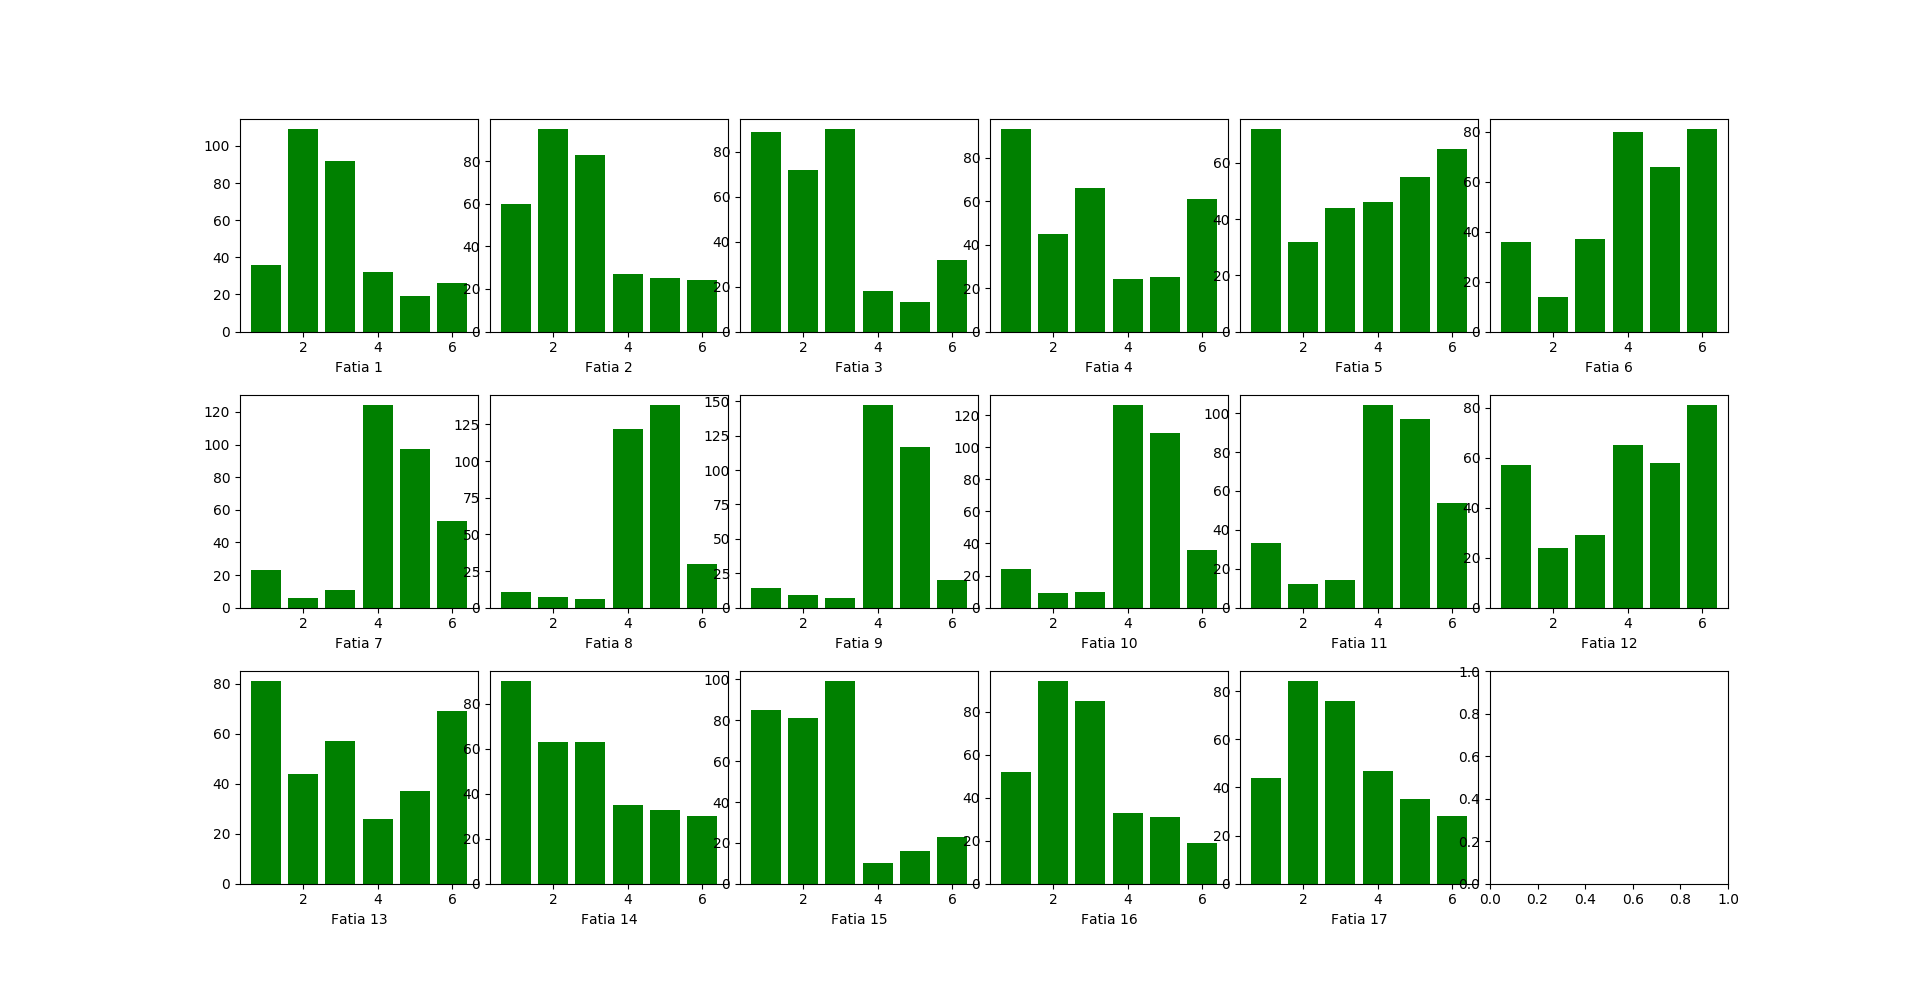
\includegraphics[width=2.5in]{imgs/antes_shuffle}
\caption{Distribuição dos dados antes do shuffle}
\label{fig:antes_shuffle}
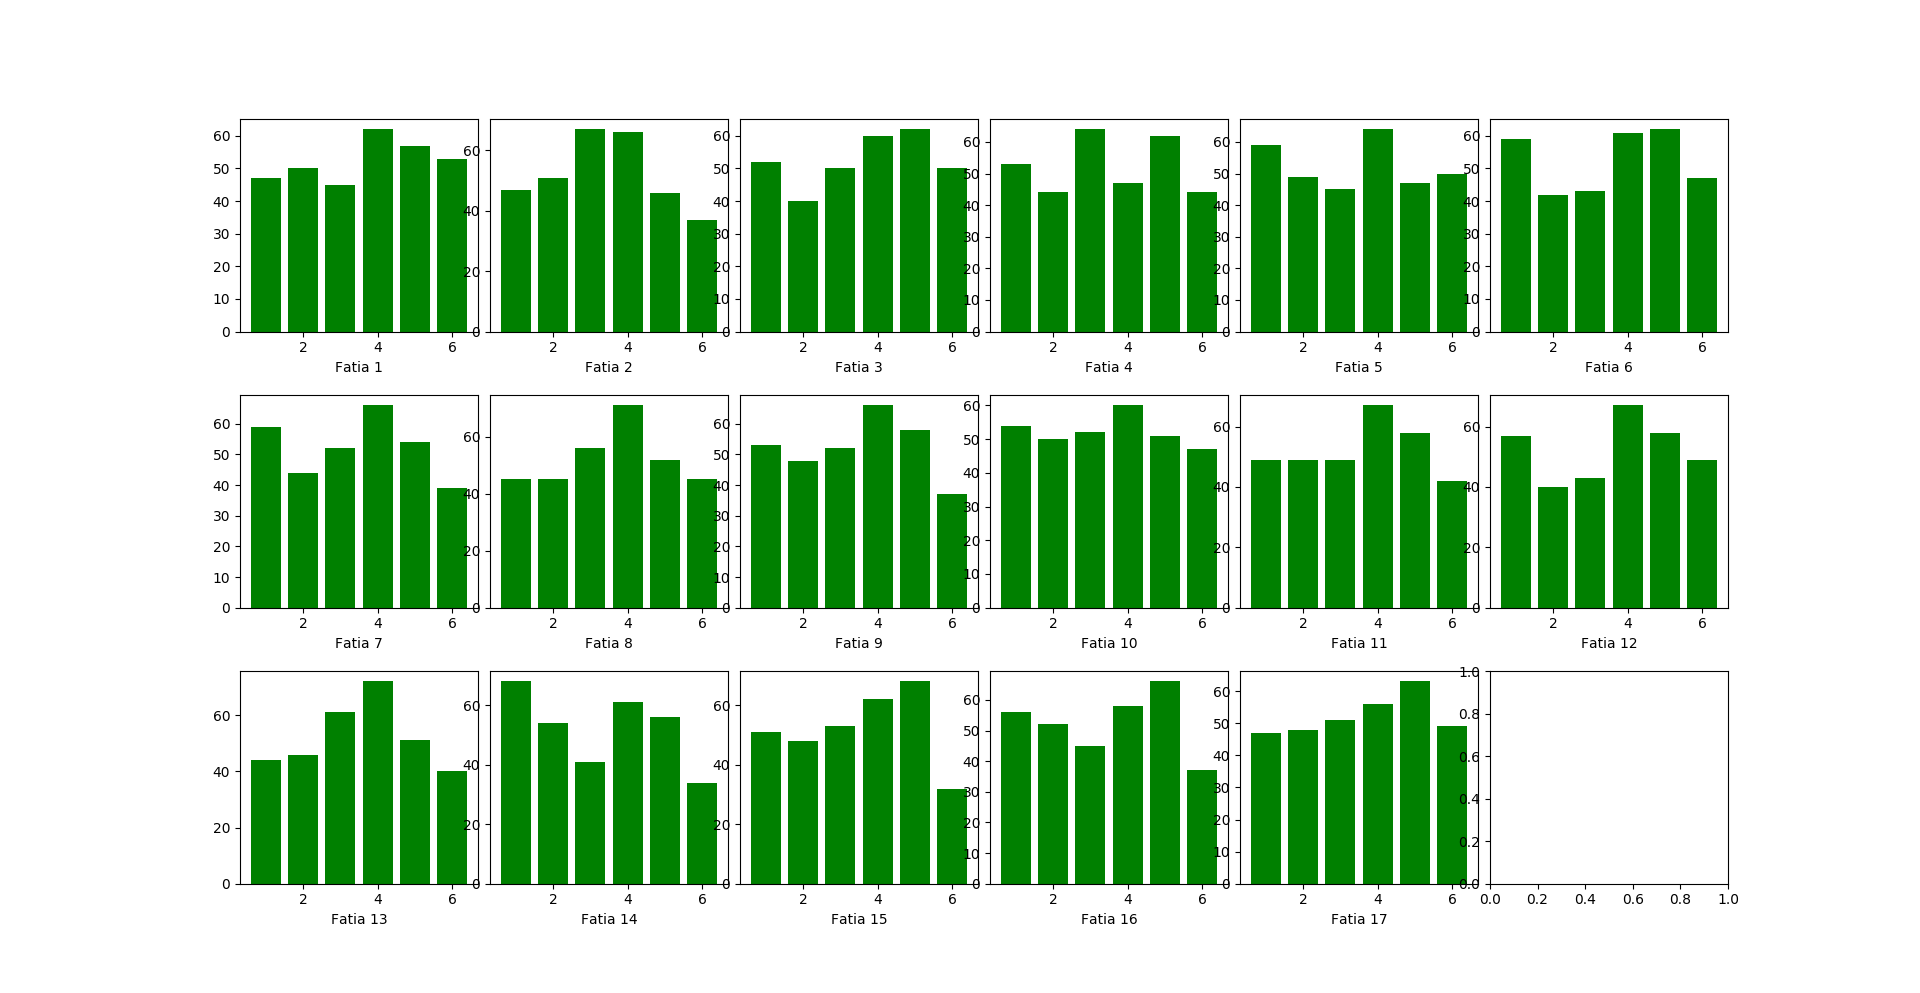
\includegraphics[width=2.5in]{imgs/apos_shuffle}
\caption{Distribuição dos dados depois do shuffle}
\label{fig:apos_shuffle}
\end{figure}

\section{Metodologia Experimental}\label{sec:metodologia}
\subsection{Sistema de Avaliação}\label{subsec:sistema_avaliacao}
%Divisões entre treinamento e teste
A fim de conseguir avaliar o desempenho de predição dos diferentes modelos 
de Aprendizado de Máquina sobre a base de dados fornecida, decidimos utilizar 
a técnica de \textsl{10-Fold Cross Validation} que é ideal para adequar os 
dados de treinamento e teste. Para isso, dividimos a quantidade total de 
amostras por $10$ e portanto, teremos $10$ \textsl{folds} (fatias) dos dados 
com tamanhos iguais. Para cada fatia N indo de $1$ a $10$, deixamos a atual 
sendo utilizada para uma partição de teste e o restante é utilizado como partição 
de treinamento, semelhante ao descrito em [3]\todo{ref}. Se uma partição de 
teste não fosse utilizada para a definição dos parâmetros, possivelmente 
teríamos um valor de F-medida máximo gerado por \textsl{overfitting} da própria 
partição de treinamento. Analogamente, deixar mais \textsl{folds} para teste e
menos para treinamento faria com que a capacidade de generalização dos modelos
pudesse ser melhor avaliada, mas em contrapartida menos dados seriam usados para
a hipótese, o que poderia diminuir sua F-medida consideravelmente.


Além disso, para que conseguíssemos otimizar a validação cruzada juntamente 
com a estimativa de parâmetros mais adequados para os algoritmos, utilizamos 
o \textsl{Grid Search}. Basicamente o que fazemos em todo o processo é escolher 
o valor do parâmetro que apresenta a maior F-medida para cada uma das partições 
utilizadas para teste na validação cruzada. Assim, é possível analisar todos os
resultados e escolher o \textsl{fold} que melhor otimiza todos os modelos 
utilizados no projeto através de uma média das F-medidas. Desta forma, podemos
então escolher o algoritmo que apresenta os melhores resultados para a base de
dados descrita na seção~\ref{sec:base_dados}.

Para o treinamento de algoritmos mais custosos como Redes Neurais Artificiais 
e o SVM, consideramos necessária a redução da grande quantidade inicial de 
atributos. Para isso, foi feita a matriz de correlação entre os atributos, onde
colunas da matriz cuja correlação era maior que $0.9$, menor que $-0.9$ foram 
removidas. Resultando em $170$ atributos aproximadamente de um total de $561$. 
Apesar da redução ter sido significativa, esse número ainda resultaria em 
execuções custosas para a geração de hipóteses. Posto isso, após algumas 
pesquisas e conselhos, o grupo decidiu fazer a implementação do método de 
Análise de Componentes Principais, disponível no arquivo \texttt{pca.m}, optando por manter atributos que preservam 
no mínimo $98\%$ da variância dos dados apresentados inicialmente, de maneira 
que a fidelidade das informações se mantivesse. Após feito o processo em cima 
da base de dados já normalizada, restaram $151$ atributos.


\subsection{Parâmetros e Medidas de Desempenho}
%Descrever as decisões do grupo nos que foram utilizados
Para o classificador KNN precisávamos definir uma maneira eficiente para 
encontrar o número ideal k de vizinhos para assim determinar a distância entre 
os pares. Para isso, capturamos o k, indo de 1 a 50, que atribui a melhor 
F-medida de predição ao KNN utilizando as partições de treinamento e teste 
definidos pelo \textsl{10-Fold Cross Validation}. Para a implementação do 
K-vizinhos mais próximos utilizamos vetorização em vários passos, de forma a melhorar o desempenho da execução.

A Regressão Logística contou com a variação apenas do parâmetro lambda, sendo
esta de $0$ a $10$. Isso
ocorreu principalmente pela grande quantidade de atributos usados, o que tornou
inviável a geração de atributos polinomiais. 


Para os algoritmos de Redes Neurais Artificiais existem vários parâmetros que
influenciam diretamente no funcionamento do algoritmo. O grupo optou por testar
as variações de lambda, número máximo de iterações e número de neurônios das
camadas ocultas. 

O parâmetro de maior dificuldade para definição foi o número de
neurônios das camadas ocultas porque impactava diretamente o tempo de
processamento e a qualidade de resultado. Para isso, o grupo buscou por
materiais e conselhos que pudessem ajudar e, a partir disso, definimos três
variações de neurônios: 
    \begin{description}
        \item[75]{Aproximadamente metade dos atributos. Esperava-se que a
        acurácia para este parâmetro fosse mais baixa.}
        \item[151]{Iguala o número de atributos depois da aplicação da Análise
        de Componentes Principais.}
        \item[300]{Esperava-se que este parâmetro, combinado com o lambda certo,
        resultasse na melhor acurácia possível apesar do alto cuso
        computacional}
    \end{description}

Para as RNA de apenas uma camada, o número máximo de iterações variou entre 200,
500 e 700. Já para as de duas camadas, este parâmetro variou entre 500, 750 e
1000.

A variação do lambda foi também um ponto de dificuldade para o caso específico
de lambda igual a 0. Isso ocorreu porque, entre os cálculos do método, o custo
acabava se tornando um NaN (Not a Number) e fazia com que o método divergisse.
Para corrigir este problema, implementou-se uma verificação que, sempre que o
cálculo do custo resultasse em um NaN, era adicionado um número suficientemente
próximo de zero ao valor, desssa forma tornando possível a computação sem
maiores problemas.

Devido a grande quantidade de funções de Kernel e diferentes parâmetros para a técnica de classificação de Máquinas de Vetores de Suporte, foram escolhidos parâmetros que mais sintetizam nosso conjunto de dados. Primeiramente, para montar o grid com os valores ótimos para cada fold da técnica de 10-Fold Cross Validation, iteramos os parâmetros C (responsável pela largura da margem) e Gamma (Parâmetro do kernel RBF, Radial Basis Function) exponencialmente.
Esta interação ocorreu da seguinte forma: para o parâmetro C, a interação ocorreu dos valores: $2^(-3)$ até $2^4$. Valores maiores que isso ultrapassaram o número máximo de interações da função svmtrain. Para o parâmetro Gamma do kernel RBF, o alcance foi entre $2^{-15}$ até $2^3$.
Também, além de utilizarmos o Kernel RBF para montar o grid, montamos um grid separado para visualizar como o SVM se comportaria com um Kernel linear, e após constatarmos que a nossa base dados não é linear, e analisarmos o grid resultante do Kernel linear, descartamos este método de classificação, por sua F-medida ser inferior a todos os outros métodos.
Como foi descrito anteriormente, o grid com os valores ótimos para cada K da técnica de K-Fold precisavam de dois parâmetros, C e Gamma, tornando o grid de três dimensões. Para contornar esta dificuldade, na qual ia dificultar a visualização dos dados, montamos a matriz com dimensões de 10 x 152, onde 10 representa a técnica de 10-Fold Cross Validation, e 152 representa as 8 interações possíveis de C multiplicadas por 19 interações possíveis de Gamma. Com isso, cada coluna seria uma combinação possível de valores de C e Gamma, mantendo sua visualização em duas dimensões.



\section{Resultados}\label{sec:resultados}
%Colocar muitas tabelas e gráficos de comparação para mostrar os resultados de predição de cada algoritmo
De acordo com a estrutura do nosso grid, primeiramente recuperamos os valores 
de parâmetros, descritos na seção \ref{sec:metodologia}, que apresentam melhor 
F-medida para cada fold da validação cruzada. As melhores F-medidas resultantes 
deste processo podem ser visualizadas na tabela \ref{fmedidas}. Como pode 
ser conferido, a melhor F-medida média foi detectada para o fold <X> e 
portanto, estabelecemos que esse é o fold ideal para todos os modelos. A partir 
disso, podemos utilizar os melhores valores dos parâmetros de cada modelo em 
relação ao fold <X>. Os parâmetros definidos podem ser visualizados na tabela
\ref{parametros}. É necessário salientar que para redes neurais, talvez a 
qualidade seja afetada positivamente ou negativamente, pois os pesos para o 
cálculo dos neurônios é totalmente aleatório em cada execução.

Após feita a seleção dos melhores parâmetros para cada classificador como foi 
descrito anteriormente, fizemos uma análise do desempenho de cada um dos 
algoritmos através das seguintes métricas: F-medida, precisão, revocação, 
acurácia e por fim, tempo de execução. A precisão e a revocação que geraram 
os F-medidas, foi uma realizada através da média da precisão e revocação de 
todas as classes, já que temos seis. Nossos dados estão poucos desbalanceados, 
como vimos do pré-processamento, então a acurácia possivelmente também 
representa valores, que em sua maioria, são verídicos. O tempo de execução 
no Octave foi recuperado através dos comandos complementares tic() e toc(), 
que disparam um timer no início da execução do algoritmo e registram o tempo 
total no final [5]\todo{ref}. Todos esses valores podem ser visualizados de forma mais 
representativa na tabela \ref{metrica_otimos}.

Além disso, geramos as curvas de aprendizado para cada um dos métodos para
mensurar o que há ou não de errado e poder refletir a respeito de medidas de
correção para aumentar o desempenho de cada método. 

\begin{table}[!t]
% increase table row spacing, adjust to taste
\renewcommand{\arraystretch}{1.3}
\caption{Melhores F-medidas (em \%) dos modelos para cada \textsl{fold}}
\label{fmedidas}
\centering
% Some packages, such as MDW tools, offer better commands for making tables
% than the plain LaTeX2e tabular which is used here.
    \begin{tabular}{|l|c|c|p{0.9cm}|p{0.9cm}|c|p{0.8cm}|}
    \hline
    & KNN & RL & RNA 1 camada & RNA 2
    camadas & SVM & F-medida média\\
    \hline
    Fold-1 & 94.724 & 88.494 & 91.490 & 91.550 & 92.608 & 91.773 \\ 
    Fold-2 & 94.143 & 86.479 & 90.448 & 89.761 & 92.482 & 90.662 \\
    Fold-3 & 93.295 & 86.614 & 91.124 & 90.591 & 92.418 & 90.808 \\ 
    Fold-4 & 94.210 & 89.510 & 92.937 & 94.333 & 96.104 & 93.418 \\ 
    Fold-5 & 93.806 & 87.193 & 92.426 & 93.165 & 93.573 & 92.326 \\ 
    Fold-6 & 94.773 & 86.931 & 92.275 & 92.108 & 93.839 & 91.985 \\ 
    Fold-7 & 95.132 & 86.979 & 92.024 & 93.397 & 92.495 & 92.005 \\ 
    Fold-8 & 92.573 & 84.634 & 91.218 & 92.393 & 92.976 & 90.758 \\ 
    Fold-9 & 94.307 & 85.959 & 91.222 & 91.613 & 93.750 & 91.370 \\ 
    Fold-10 & 94.010 & 89.633 & 91.750 & 92.425 & 93.455 & 92.255 \\
    \hline
    \end{tabular}
\end{table}


\begin{table}[!t]
% increase table row spacing, adjust to taste
\renewcommand{\arraystretch}{1.3}
\caption{Métrica dos classificadores utilizando os parâmetros ótimos}
\label{metrica_otimos}
\centering
\begin{tabular}{|p{1.8cm}|c|c|p{1cm}|p{1cm}|c|}
\hline
    & KNN & RL & RNA 1 camada & RNA 2
    camadas & SVM\\
\hline
F-medida (\%) & 94.210 & 89.141 & 91.997 & 93.501 & 95.521 \\
Precisão (\%) & 94.060 & 89.126 & 91.813 & 93.320 & 95.346 \\
Revocação (\%) & 94.360 & 89.156 & 92.183 & 93.684 & 95.696 \\
Acurácia (\%) & 93.996 & 88.930 & 91.932 & 93.433 & 95.497 \\
Tempo de Execução (em segundos) & 59.924 & 14.660 & 208.183 & 1025.951 & 10.029 \\
\hline
\end{tabular}
\end{table}


\begin{figure}[!t]
\centering
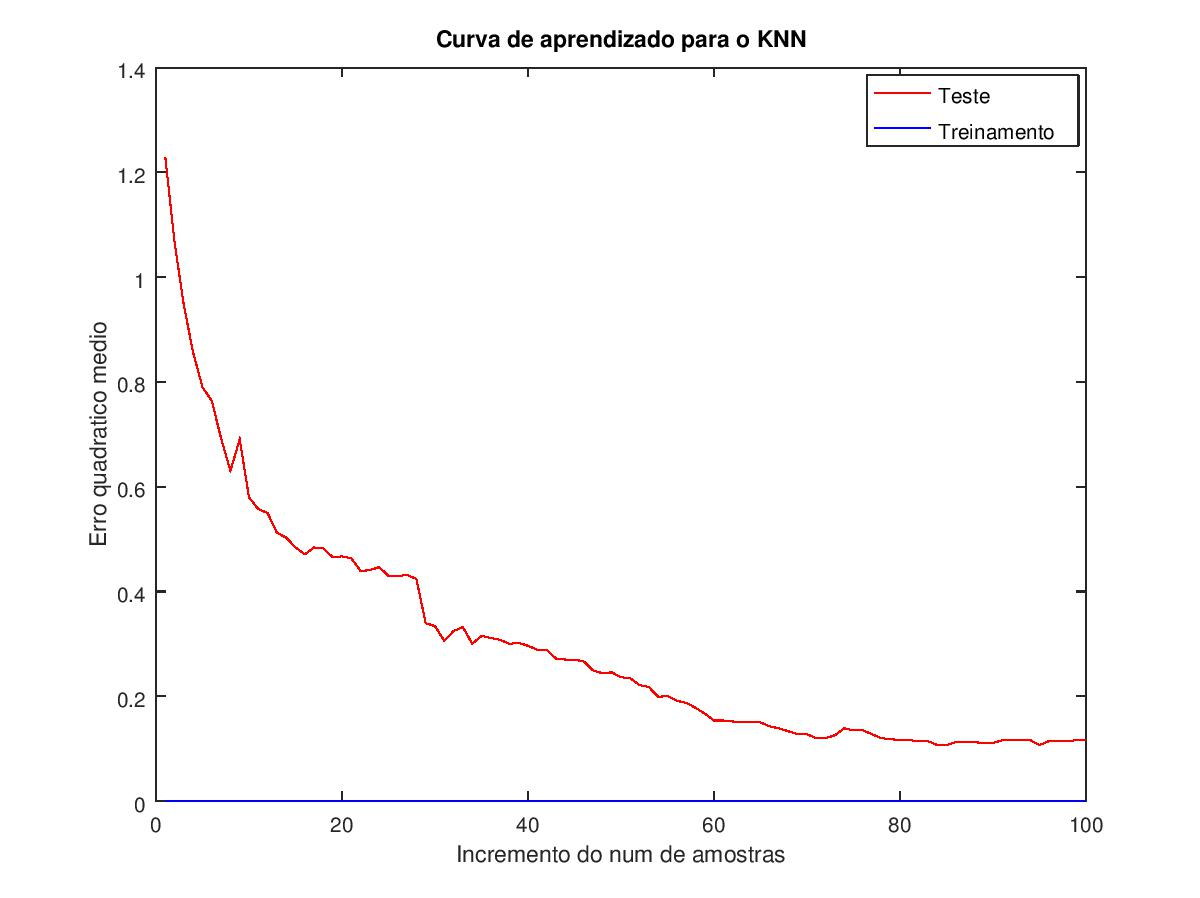
\includegraphics[width=2.5in]{imgs/KNNcurve}
\caption{Curva de Aprendizado para o método KNN}
\label{fig:knn_curve}
\end{figure}

\begin{figure}[!t]
\centering
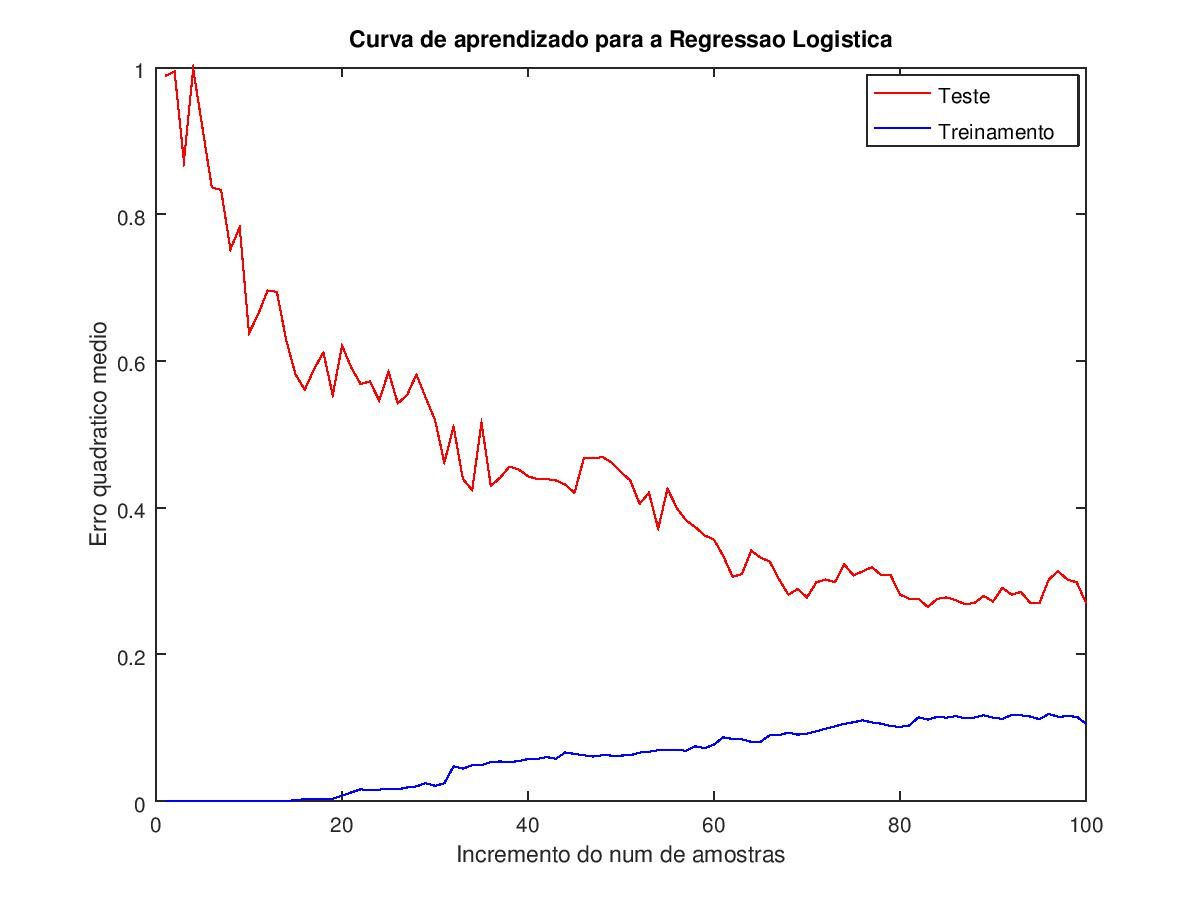
\includegraphics[width=2.5in]{imgs/RLcurve}
\caption{Curva de Aprendizado para o método de Regressão Logística}
\label{fig:rl_curve}
\end{figure}

\begin{figure}[!t]
\centering
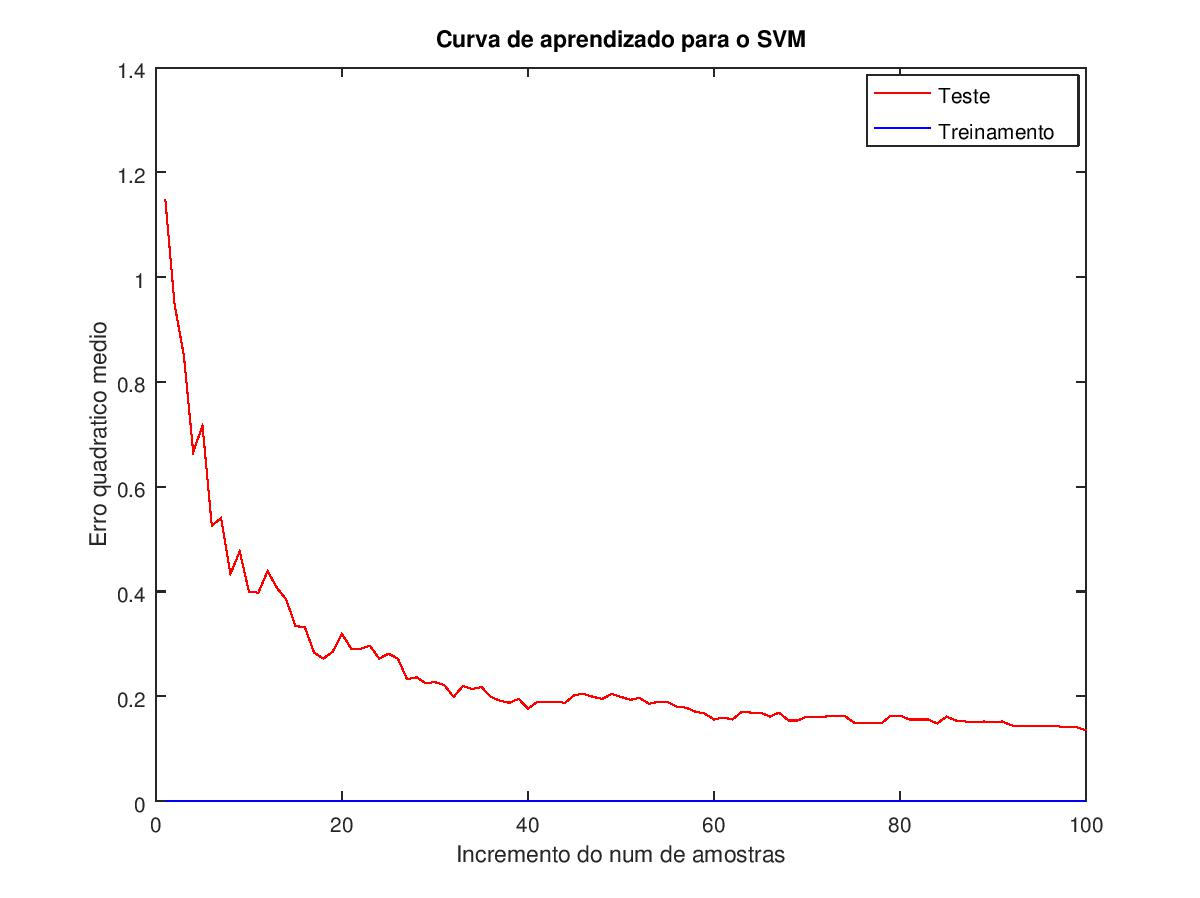
\includegraphics[width=2.5in]{imgs/SVMcurve}
\caption{Curva de Aprendizado para o método SVM}
\label{fig:svm_curve}
\end{figure}

\section{Conclusões}\label{sec:conclusao}
Antes de mais nada, gostaríamos de frisar a importância do pré-processamento no aprendizado de máquina, pois sem ele, ou com sua aplicação de forma errônea, a porcentagem de acerto do modelo final vem a ser bem baixa.
    Em seguida, o processo de tuning dos algoritmos através da formação do grid search é computacionalmente exaustivo, porém completamente necessário para que se encontre os parâmetros ótimos para a geração de um bom modelo. Infelizmente, mesmo com todos os processos realizados, presenciamos a geração de overfitting em vários modelos quando comparados com a base de treinamento, ou seja, com amostras já conhecidas. Acreditamos que um dataset com mais amostras pudesse reduzir a variância dos erros e otimizar de maneira mais precisa a classificação, porém este passo não estava ao nosso alcance neste projeto.
    Por fim, após o grupo gerar as hipóteses com diferentes algoritmos de aprendizado, pode-se observar que especificamente para essa base de dados, o modelo criado pela Máquina de Vetores de Suporte conseguiu gerar o melhor modelo de predição, resultando em uma F-medida média de 95.5\% na classificação das amostras de teste. De maneira geral, nosso resultado foi satisfatório. Como citado por [2]\todo{ref}, que apresenta a aplicação do SVM em uma base muito próxima à utilizada neste projeto e que utilizou um pré-processamento mais simples, a performance do SVM na base de teste ficou entre 90\% e 96\%.

\section{Referências}
\todo[inline]{ajeitar o .bib de referências}

\clearpage
\appendix
\section{Execução do projeto}\label{apendice_execucao}
%Passo-a-passo para obter os resultados no Octave que foram detalhados no relatório
Para que a execução do projeto ocorra de forma ideal, é necessário que a 
hierarquia de pasta de todos os arquivos seja mantida da maneira em que fora 
entregue, sem mudanças de diretório.

É necessário também que haja a biblioteca libsvm para a execução do algoritmo 
de máquina de vetores de suporte, o projeto já fornece a biblioteca compilada 
para o sistema operacional Windows (32/64bits) e para o Linux (64bits). 
Caso pretenda executar em um sistema operacional diferente, será necessário 
compilar e adicionar a biblioteca ao path do Octave/Matlab antes de executar o 
projeto, para mais informações, o link do repositório se encontra aqui: https://github.com/cjlin1/libsvm.\todo{ref}

Além da biblioteca para o algoritmo SVM, ainda em trechos de código de Redes 
Neurais Artificiais, utilizamos dos pacotes io e statistics do próprio Octave. 
Para o cálculo dos erros quadráticos e o plot dos gráficos de curvas de 
aprendizado também fazemos uso do pacote image do Octave. É necessário que 
seja feita a instalação dos mesmos da maneira que é descrito em https://octave.org/doc/v4.2.1/Installing-and-Removing-Packages.html. 

Inicialmente, fornecemos os dados com um pré-processamento já aplicado que 
foram gerados e gravados no arquivo de nome pre\_processed.mat. Porém, se por 
algum motivo for necessário fazer o pré-processamento novamente, é necessário 
executar no Octave/Matlab o arquivo preprocessing.m que utiliza os arquivos da 
base de dados inicial fornecidos no diretório dataset\_uci. Vale a pena 
ressaltar que toda vez que o pré-processamento é executado, ocorre um novo 
shuffle nos dados, tal qual pode alterar razoavelmente os resultados aqui apresentados.

Para visualizar e/ou executar os testes feitos pelo grupo com a formação do 
grid search e 10-fold cross validation, é necessário que seja feita a execução 
do arquivo exec\_project.m. É importante alertar que a execução deste arquivo 
completo pode vir a demorar mais de 24h por se tratar de um código que passa 
por muitas iterações.

Para visualizar e/ou executar o resultado dos classificadores com os parâmetros
ótimos já selecionados, de maneira a entender a qualidade apresentada por cada 
um através da F-medida, é necessário que seja feita a execução do arquivo 
optimized\_project.m.
A geração das curvas de aprendizado como descritas na seção
\ref{sec:resultados} estão contidas no arquivo learning\_curves.m.




% An example of a floating figure using the graphicx package.
% Note that \label must occur AFTER (or within) \caption.
% For figures, \caption should occur after the \includegraphics.
% Note that IEEEtran v1.7 and later has special internal code that
% is designed to preserve the operation of \label within \caption
% even when the captionsoff option is in effect. However, because
% of issues like this, it may be the safest practice to put all your
% \label just after \caption rather than within \caption{}.
%
% Reminder: the "draftcls" or "draftclsnofoot", not "draft", class
% option should be used if it is desired that the figures are to be
% displayed while in draft mode.
%
%\begin{figure}[!t]
%\centering
%\includegraphics[width=2.5in]{myfigure}
% where an .eps filename suffix will be assumed under latex, 
% and a .pdf suffix will be assumed for pdflatex; or what has been declared
% via \DeclareGraphicsExtensions.
%\caption{Simulation Results}
%\label{fig_sim}
%\end{figure}

% Note that IEEE typically puts floats only at the top, even when this
% results in a large percentage of a column being occupied by floats.


% An example of a double column floating figure using two subfigures.
% (The subfig.sty package must be loaded for this to work.)
% The subfigure \label commands are set within each subfloat command, the
% \label for the overall figure must come after \caption.
% \hfil must be used as a separator to get equal spacing.
% The subfigure.sty package works much the same way, except \subfigure is
% used instead of \subfloat.
%
%\begin{figure*}[!t]
%\centerline{\subfloat[Case I]\includegraphics[width=2.5in]{subfigcase1}%
%\label{fig_first_case}}
%\hfil
%\subfloat[Case II]{\includegraphics[width=2.5in]{subfigcase2}%
%\label{fig_second_case}}}
%\caption{Simulation results}
%\label{fig_sim}
%\end{figure*}
%
% Note that often IEEE papers with subfigures do not employ subfigure
% captions (using the optional argument to \subfloat), but instead will
% reference/describe all of them (a), (b), etc., within the main caption.


% An example of a floating table. Note that, for IEEE style tables, the 
% \caption command should come BEFORE the table. Table text will default to
% \footnotesize as IEEE normally uses this smaller font for tables.
% The \label must come after \caption as always.
%
%\begin{table}[!t]
%% increase table row spacing, adjust to taste
%\renewcommand{\arraystretch}{1.3}
% if using array.sty, it might be a good idea to tweak the value of
% \extrarowheight as needed to properly center the text within the cells
%\caption{An Example of a Table}
%\label{table_example}
%\centering
%% Some packages, such as MDW tools, offer better commands for making tables
%% than the plain LaTeX2e tabular which is used here.
%\begin{tabular}{|c||c|}
%\hline
%One & Two\\
%\hline
%Three & Four\\
%\hline
%\end{tabular}
%\end{table}


% Note that IEEE does not put floats in the very first column - or typically
% anywhere on the first page for that matter. Also, in-text middle ("here")
% positioning is not used. Most IEEE journals/conferences use top floats
% exclusively. Note that, LaTeX2e, unlike IEEE journals/conferences, places
% footnotes above bottom floats. This can be corrected via the \fnbelowfloat
% command of the stfloats package.



%\section{Conclusion}
%The conclusion goes here. this is more of the conclusion

% conference papers do not normally have an appendix


% trigger a \newpage just before the given reference
% number - used to balance the columns on the last page
% adjust value as needed - may need to be readjusted if
% the document is modified later
%\IEEEtriggeratref{8}
% The "triggered" command can be changed if desired:
%\IEEEtriggercmd{\enlargethispage{-5in}}

% references section

% can use a bibliography generated by BibTeX as a .bbl file
% BibTeX documentation can be easily obtained at:
% http://www.ctan.org/tex-archive/biblio/bibtex/contrib/doc/
% The IEEEtran BibTeX style support page is at:
% http://www.michaelshell.org/tex/ieeetran/bibtex/
\bibliographystyle{IEEEtran}
% argument is your BibTeX string definitions and bibliography database(s)
%\bibliography{IEEEabrv,../bib/paper}
\bibliography{IEEEfull}
%
% <OR> manually copy in the resultant .bbl file
% set second argument of \begin to the number of references
% (used to reserve space for the reference number labels box)
%\begin{thebibliography}{1}

%\bibitem{IEEEhowto:kopka}
%H.~Kopka and P.~W. Daly, \emph{A Guide to \LaTeX}, 3rd~ed.\hskip 1em plus
%  0.5em minus 0.4em\relax Harlow, England: Addison-Wesley, 1999.

%\end{thebibliography}




% that's all folks
\end{document}


